\documentclass[thesis]{cluu}

\usepackage[style=cluu]{biblatex}
\usepackage{tabularx}
\usepackage[acronym]{glossaries}
\usepackage{tikz}
\usetikzlibrary{arrows.meta,positioning,shapes.geometric,fit}
\usepackage{cleveref}
\usepackage{graphicx}
\graphicspath{ {./images/} }
\usepackage{adjustbox}

% Define tikz styles to reuse in figures
\usepackage[edges]{forest}
\usetikzlibrary{arrows.meta} % for Latex arrowheads

%this has to be the last 
\usepackage{hyperref}

\usepackage{silence}
\WarningFilter{biblatex}{Package option 'sortcites' enabled}
%Package biblatex: Package option 'sortcites' enabled.
%(biblatex)	Verify postnote placement
%\usepackage[nameref]


\makeglossaries

\newacronym{ai}{AI}{Artificial Intelligence}
\newacronym{ml}{ML}{Machine Learning}
\newacronym{cv}{CV}{cross-validation}
\newacronym{nlp}{NLP}{Natural Language Processing}
\newacronym{call}{CALL}{Computer-Assisted Language Learning}
\newacronym{icall}{icall}{Intelligent CALL}
\newacronym{capt}{CAPT}{Computer-Assisted Pronunciation Training}
\newacronym{json}{JSON}{JavaScript Object Notation}
\newacronym{llm}{LLM}{Large Language Model}
\newacronym{nlg}{NLG}{Natural Language Generation}
\newacronym{md}{MD}{Mispronunciation Detection}
\newacronym{mdd}{MDD}{Mispronunciation Detection and Diagnosis}
\newacronym{ctc}{CTC}{Connectionist Temporal Classification}
\newacronym{cnn}{CNN}{Convolutional Neural Network}
\newacronym{fleurs}{FLEURS}{Few-shot Learning Evaluation of Universal Representations of Speech}
\newacronym{l2}{L2}{second language}
\newacronym{l1}{L1}{first language}
\newacronym{sla}{SLA}{second-language acquisition}
\newacronym{nn}{NN}{neural network}
\newacronym{dnn}{DNN}{deep neural network}
\newacronym{tts}{TTS}{text-to-speech}
\newacronym{asr}{ASR}{automatic speech recognition}
\newacronym{ipa}{IPA}{the International Phonetic Alphabet}
\newacronym{g2p}{G2P}{grapheme-to-phoneme}
\newacronym{wals}{WALS}{the World Atlas of Linguistic Structure}
\newacronym{mfa}{MFA}{Montreal Forced Aligner}
\newacronym{mt}{MT}{Machine Translation}
\newacronym{tl}{TL}{Transfer Learning}
\newacronym{mooc}{MOOC}{massive open online course}
\newacronym{e2e}{E2E}{end-to-end}
\newacronym{gop}{GOP}{goodness of pronunciation}
\newacronym{gmm}{GMM}{Gaussian Mixture Model}
\newacronym{hmm}{HMM}{Hidden Markov model}
\newacronym{cer}{CER}{character error rate}
\newacronym{wer}{WER}{word error rate}
\newacronym{per}{PER}{phone error rate}
\newacronym{rover}{ROVER}{Recognizer Output Voting Error Reduction}
\newacronym{ssml}{SSML}{Speech Synthesis Markup Language}
\newacronym{nltk}{NLTK}{Natural Language Toolkit}
\newacronym{loso}{LOSO}{leave-one-speaker-out}
\newacronym{s2s}{Seq2Seq}{sequence-to-sequence}
\newacronym{dpad}{DPAD}{diversified and preference-aware decoding}
\newacronym{p2p}{P2P}{phoneme-to-phoneme}

\forestset{
  box/.style={
    draw, rounded corners=2mm, thick,
    minimum height=9mm, align=center
  },
  internal/.style={box, fill=blue!10},
  posleaf/.style={box, fill=green!15},
  negleaf/.style={box, fill=red!15},
  edgelabel/.style={midway, sloped, above},
}

% Define a new counter for paragraphs (delete when paper is done)
\newcounter{paranum}
% Command to increment and display the paragraph number for initial planning
\newcommand{\numberedparagraph}{\par\refstepcounter{paranum}\textbf{[\theparanum] }}

\newcommand{\todo}[1]{\textcolor{red}{#1}}

% use Doulos SIL for IPA transcriptions
\newfontfamily\ipafont{Doulos SIL}[Scale=MatchLowercase]
\newcommand{\ipa}[1]{{\ipafont #1}}

% research questions for referencing
%\newcommand{\researchquestion}[3]{%
%  \refstepcounter{section}
%  \label{#1}%
%  \textbf{RQ\thesection.} #2%
%  \expandafter\gdef\csname #1text\endcsname{#2}%
%}

% Usage
%\researchquestion{rq:1}{How effective are state of the art ASR
%systems in detecting pronunciation errors in adult, English-speaking
%Ulster Irish learners?}{}



% ThesisProject is auto updated by zotero
\addbibresource{ThesisProject.bib}

\begin{document}
\title{Low-Resource CAPT: An Irish Perspective} % crap title, workshop this
\author{Peter Cady}
% \date{...}
\supervisors{Johan Sjons, Uppsala University\\
  Jim O' Regan, KTH Royal Institution of Technology}
% Use \supervisor (without s at end) if you have only one

\maketitle

\begin{abstract}
    \numberedparagraph{summarize the motivation}
    \numberedparagraph{problem overview}
    \numberedparagraph{experiment}
    \numberedparagraph{main findings and contributions.}
\end{abstract}

\tableofcontents

\addchap{Preface}
% with \addchap instead of \chapter it isn't numbered.
\addchap{Acknowledgements}
Thank my partner
Thank Johan
I would especially like to thank Jim O' Regan for all his thought-provoking insights, encouragement, and advice, which were crucial for me getting my bearings in a project which pushed me to grow well beyond my limits. The process was deeply meaningful to me. Thank you.
Thank Greg
I would like to thank my Irish professor Gregory Darwin for his commitment and engagement in promoting Irish literature and the Irish language 
Thank examiner

\printglossary[type=\acronymtype]

\printglossary

\chapter{Introduction}
\numberedparagraph{Lead work here. Outline modern context of minority languages in nlp. Introduce Irish context in this framework.}
\todo{revisit introduction, try to lead with an impactful framing of the motivation of the work.}
Language competency is crucial for securing opportunities in the workplace as well as for accessing services and exercising rights in society at large. As our surroundings become ever more digitally interconnected, these interactions are increasingly mediated by language technologies, for both good and ill. Such technologies are often identified as promising tools to promote language use and language learning, but are also implicated in the coalescence of online interaction around a few dominant languages such as English, complicating the glowing promises often offered by their proponents. Low-resource language communities struggle to keep pace with the most recent technological advancements given the relative scarcity of resources they are faced with, necessitating approaches tailored to these limitations if the true promise of cutting-edge language technologies is to be realized for these groups most in need. The momentum of the pre-training/fine-tuning paradigm within \gls{asr} and \gls{ml} more generally in recent years offers a glimmer of hope to those working toward making accessible tools for such communities, enabling the use of more plentiful data to support tools for languages facing varying levels of resource scarcity.

\numberedparagraph{Reiterate need for a solution, lead into research questions.} 
Promoting speech technologies for language learning could be of particular benefit for languages such as Irish which struggle to propagate native models of speech effectively to motivated learners outside of traditionally Irish-speaking areas. Through \gls{capt} applications built with careful use of the aforementioned, we might find the scaleable, resource con

\numberedparagraph{RQ's} 
To this end, in this work we explore two potential avenues to overcoming the data limitations faced by Irish and other languages like it: one, by using the data we \textit{do} have by harnessing readily available monolingual data in a model ensemble; and the other, by imitating the data we \textit{wish} we had with \gls{tts}-generated learner approximations to train a model with. These approaches are formulated concretely as:
\begin{enumerate}
  \item To what extent can a resource-conscious ensemble of monolingual ASR models (Irish and English) approach the performance of a high-resource upper-bound model trained on fully annotated mispronunciation data (L2-ARCTIC)?\label{rq:1}
  \item To what extend can a model trained on TTS-generated synthetic mispronunciation data approach the performance of a high-resource upper-bound trained on fully annotated learner mispronunciation data (L2-ARCTIC)?\label{rq:2}
\end{enumerate}



\numberedparagraph{Outline key goals of thesis, give a "road map" for what's to come.}
In this thesis we explore the feasibility of two primary methods of overcoming the scarcity of phonetically annotated \gls{l2} Irish learner data for \gls{md} applications. One approaches the problem with ensembles of monolingual \gls{asr} models for which data scarcity less acute, and another using a schema of data generation by leveraging established \gls{tts} systems to approximate learner speech: a potential low-cost alternative to large-scale phonetic annotation. By exploring these approaches, we aim to illuminate possible ways forward for low-resource language communities interested in developing automated technologies for language learning and pronunciation training.


\chapter{Background}
\numberedparagraph{Short overview of background section}

In the following section we will outline the context motivating our current work with relation to \gls{nlp} and \gls{asr} research for minority languages. We begin by summarizing the state of minority languages in current research, highlighting some promising trends as well as some thusfar recalcitrant problems hindering more equal access to the benefits of our time's rapid advances in language technology. We then proceed to outline the more general research space of the current work: \gls{call} and \gls{capt} before digging into the core task of \gls{capt} systems: \gls{md} and \gls{mdd}. We conclude with a technical overview of modern \gls{asr} systems used for such tasks, leaving the specific efforts of researchers to overcome data limitation inherent to low-resource languages in the next section, \todo{get chapter and section references working}%\nameref{chap:Related Work}.

\section{Irish \& The Predicament of Minority Languages in \acrfull{nlp}}\label{back:lr-lang}

\numberedparagraph{introduce need for general-use systems.}

Developing language technologies that can scale beyond the language they are designed for is no new goal for \gls{nlp} research. The value of such a property is apparent: transferring an existing system seamlessly to another language could potentially save significant resources for language communities without the ability to fund such system development themselves. Actually achieving this goal in practice, however, is no simple endeavor, typically requiring some level of linguistic awareness which is all-to-often lamentably absent \parencite[see][inter alia]{benderAchievingEvaluatingLanguageIndependence2011,joshiStateFateLinguistic2021,hedderichSurveyRecentApproaches2021}. For example, success in applying word-based n-gram approaches to a language rests on the language's level of inflectional morphology: the lower the better. Higher morphological complexity together with variations in word order raise data sparsity problems which n-gram approaches rooted in English struggle to handle \parencite{benderAchievingEvaluatingLanguageIndependence2011}. This should come as no surprise, given the relatively fixed word order and low levels of inflectional morphology present in English, but it illustrates a need for caution: systems developed for a given language may make implicit assumptions about language structure which do not generalize well.\todo{add concrete example to illustrate? maybe exemplify more directly from above reference} Linguistic typology can provide important clues as to what features are shared between the original development language and possible languages of extension for a system. Information of this kind has, for many of the worlds languages, already been gathered by linguists. Perhaps the most renowned database of typological information is \gls{wals} \parencite{matthewdryerWorldAtlasLanguage2024}, a free, online resource currently boasting 152 chapters with detailed descriptions of 192 linguistic features spanning over 2,600 of the world's languages. By explicitly mobilizing linguistic knowledge already painstakingly gathered by linguistic typologists, we can identify where languages agree, where they differ, and hopefully identify some of the implicit, ungeneralizable assumptions that have hindered past efforts to create more accessible language technologies.

\numberedparagraph{language disparity in lang tech.} 
Despite claims of language-agnostic systems often touted by proponents of emerging \gls{ai} systems, these have often also fallen well short of such promise \parencite{benderAchievingEvaluatingLanguageIndependence2011}\todo{add some examples of where to read further + inter alia}. The overwhelming majority of the world's languages still have no footprint in emerging language technologies \parencite{joshiStateFateLinguistic2021}. In the past, building \gls{nn}-based language technologies demanded immense quantities of labeled data: a high bar of entry to the language communities of those languages with limited if any access to such resources, and an ongoing issue which continues to stimulate a body of research dedicated to overcoming it \parencite[see][for an overview]{magueresseLowresourceLanguagesReview2020}. For languages where data availability is no obstacle, research and development can proceed unfettered by the prohibitive cost of curating datasets from scratch. As our daily lives grow increasingly integrated with the digital realm, language communities without the same support are obliged to switch to more digitally dominant languages (often English) to gain access to these new resources, narrowing the opportunities to engage with resources and services through the medium of their community language \parencite{nichasaideCanWeDefuse2019}. A particularly sobering taxonomy illustrating the states of languages facing such disparities is formulated by \textcite{joshiStateFateLinguistic2021} and reproduced in \Cref{tab:data_availability}, which outlines the challenges faced by languages in resource terms in the digital space, and how dominant a small group of languages are within it. Those at the bottom of the data availability scale at level 0, 'The Left-Behinds' have virtually no data of any kind available to support language technology development. those in the middle at level 2 or 3 have some resources, net presence, and/or research communities supporting them, but critically lack in substantial quantities of the labeled data typically required for cutting-edge \gls{nlp} tools. At the top, languages like English reap the lion's share of overall investment and development. Of particular note for the privileged few that find themselves at the top of the heap is their typological similarity, being drawn as they are from a few dominant language families (and even dominant branches within these larger families). This state of affairs constitutes a sort of typological echo-chamber for the cutting edge of \gls{nlp} developments, a point which we will return to shortly.

\begin{table}[h]
    \centering
    \begin{tabularx}{\textwidth}{|X|p{2cm}|p{1.75cm}|}
        \hline
        \textbf{Class Descriptions} & \textbf{Example Languages} & \textbf{\% of total languages}\\ \hline
        \textbf{0} The Left-Behinds: Virtually ignored in language technology. Exceptionally limited resources available, even with respect to unlabeled data. & Dahalo, Bora & 88.17\%\\ \hline
        \textbf{1} The Scraping-Bys: Some unlabeled data. With organized promotion and data collection, there is hope for improvement in coming years. & Fijian, Navajo & 8.93\%\\ \hline
        \textbf{2} The Hopefuls: Limited labeled data. Support communities help these languages survive, and there is promise for \gls{nlp} tools in the near term. & Zulu, \textbf{Irish} & 0.76\%\\ \hline
        \textbf{3} The Rising Stars: Strong web presence and thriving community online. Lacking labeled data. Good potential for \gls{nlp} tool development for these languages. & Indonesian, Hebrew & 1.13\%\\ \hline
        \textbf{4} The Underdogs: Much unlabeled data, and less but still significant labeled data. Dedicated investment from NLP communities. & Russian, Dutch & 0.72\%\\ \hline
        \textbf{5} The Winners: Dominant online presence with massive investment and resources. & English, German & 0.28\%\\ \hline
    \end{tabularx}
    \caption{Data availability \& status taxonomy of languages adapted from work by \textcite{joshiStateFateLinguistic2021}.}
    \label{tab:data_availability}
\end{table}
\numberedparagraph{set the Irish case in this context, outline challenges currently undertaken by developers}

Despite some advantages not afforded other minority languages, Irish still finds itself struggling to maintain a footing in the the digital realm, placed by \textcite{joshiStateFateLinguistic2021} in class 2 of the taxonomy in \Cref{tab:data_availability}. It enjoys ongoing investment by the Irish state, nominal status of Irish as the first national language of the Republic of Ireland, and research dedicated to its promotion \parencite[e.g. through the ABAIR initiative dedicated to developing speech technologies for Irish, see][]{chasaideABAIRInitiativeBringing2017}. At the same time, it is a typological outlier in several respects: it is a verb-initial language with relatively complex inflectional morphology, and a distinct (though still Latin-based) orthography. Features like these put Irish at odds with many languages in the high-resource echo-chamber, complicating the ability to leverage cutting-edge models to linguistic features with no representation in a model's training data. Furthermore, though we have treated Irish as a single entity thus far, an important complication reveals itself in the discontiguous nature of the Irish-speaking areas, referred to as \textit{the Gaeltacht} or \textit{the Gaeltachtaí}(pl.). Each of the three main areas (i.e. Ulster, Connacht, and Munster \ref{fig:gaeltacht}) speak markedly distinct varieties of Irish, necessitating labeled data from each variant if these groups are to be adequately serviced by new technologies \parencite{nichasaideCanWeDefuse2019}. In the face of such limitations, today's data-hungry tools simply cannot be expected to perform to the same level on languages like Irish without the necessary resources. It should be noted that the pretraining/finetuning paradigm of recent massive multilingual models does mitigate this demand for data somewhat by leveraging unlabeled cross-lingual data, reducing the need for labeled data in the language finetuned to \parencite{hedderichSurveyRecentApproaches2021,ranathungaNeuralMachineTranslation2021,joshiStateFateLinguistic2021}, but for other languages without even minimal labeled data to their name, this is a small comfort.

\begin{figure}[h]
    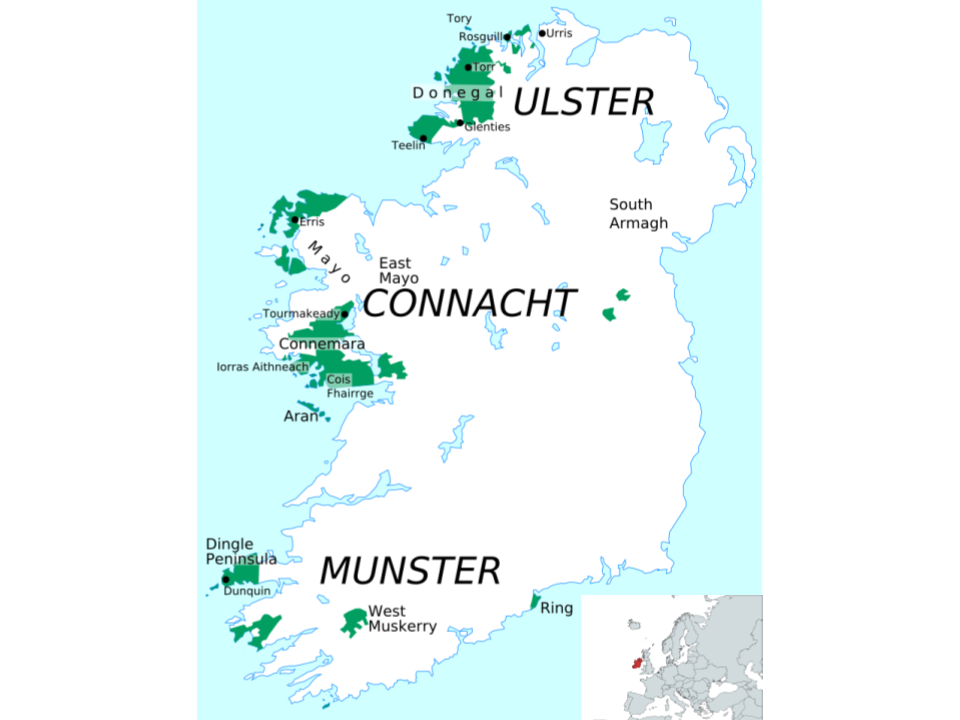
\includegraphics[width=10cm]{Gaeltachtai_with_europe_highlight_centered.png}
    \centering
    \label{fig:gaeltacht}
    \caption{Area of the Gaeltachtaí (Irish-speaking areas of Ireland) colored in green. The original uploader of the map of Ireland was Angr at English Wikipedia. - Transferred from en.wikipedia to Commons., CC BY-SA 3.0. European map was created with mapchart.net}
\end{figure} 

\numberedparagraph{problems to be solved for Irish speakers}
Though the hurdles facing the Irish language in the digital sphere are a relatively recent concern, the issues facing it in the real world are anything but. It is currently classified by UNESCO as being \textit{definitely endangered} \parencite{moseleyAtlasWorldsLanguages2010}, following centuries of varying rates of contraction due to encroachment by English \todo{give some more explanation of the history, handle with care}. Irish survives as a community languages in the aforementioned Gaeltacht areas, though even there it is estimated that only 24\% of inhabitants speak Irish on a daily basis \parencite{nichasaideSPEECHTECHNOLOGYDOCUMENTATION2015}. Despite the state of Irish as a \gls{l1}, it is comparatively strong as a \gls{l2} \parencite{broinNewUrbanIrish2014}. A growing number of parents seek Irish-medium education for their children outside the Gaeltacht, and immersive summer courses remain popolar among adults looking to learn or reconnect with the language. This encouraging \gls{l2} engagement intersects with thorny issues of supply, however, as many of the teachers are not themselves native speakers with an accompanying native grasp of the structure and sound of the language \parencite{nichasaideSPEECHTECHNOLOGYDOCUMENTATION2015,nichasaideCanWeDefuse2019}. This limited native speaker model for \gls{l2} speakers is particularly problematic for teaching pronunciation, complicating the acquisition of some sound contrasts critical to disambiguating the Irish grammar. Perhaps chiefly among these, contrasts between the secondary articulation of consonants into \textit{palatalised} and \textit{velarised} variants play an instrumental role in a number of grammatical functions, such as in the formation of certain plurals and genitive marking \parencite{snesarevaPalatalizationDublinIrish2016,gabrieleEnglishInfluenceL2,broinNewUrbanIrish2014,stensonModernIrishComprehensive2020}. Since the Roman alphabet doesn't provide symbols for this distinction, Irish orthography marks it via adjacent letters as seen in \todo{give sub-table references} of \Cref{tab:sound_contrasts}: so-called \textit{slender} vowels ('i' and 'e') around a consonant denote \textit{palatalisation}, while \textit{broad} vowels ('a', 'o', and 'u') mark \textit{velarisation}\footnote{For initial consonants, the following vowel plays the determining role, for final consonants, the preceding vowel, and for medial consonants, the vowels flanking it.} \parencite{stensonModernIrishComprehensive2020}. Mutation effects are another pervasive element of the Irish grammar relying on sound alterations, the most common of which are \textit{lenition} and \textit{eclipsis}. Lenition, traditionally termed \textit{séimhiú} (/\ipa{ˈʃeːvʲuː}/), is commonly marked with an 'h' following the lenited consonant as seen on \Cref{tab:sound_contrasts}, and originally denoted a weakening in the manner of articulation, though the relationship between consonants and their lenited versions is less immediately apparent now for some consonants \parencite{stensonModernIrishComprehensive2020}. Eclipsis, traditionally \textit{úru} (/\ipa{ˈʊɾˠuː}/), involves replacing the original consonant with a nasalized or voiced version, and is denoted by appending the new sound character before the consonant being eclipsed\ref{tab:sound_contrasts} \todo{add sub-table refs and double check if this description covers all the bases}. These and other structural underpinnings of the language can have far-reaching implications for intelligability if not adequately mastered by students. Indeed, a study undertaken by \textcite{broinNewUrbanIrish2014} reveals that realisations of phonological details like those above have error rates of over 50\% on average for urban speakers, with some as high as 82\%---a stark departure from their gaeltacht counterparts which lie below 10\%. Providing wider access to better native models of pronunciation---not to mention native models of morphology---could do much to close this gap, making mutual intelligability between gaeltacht and urban speakers more attainable. 

\begin{table}[ht]
  \centering
  \caption{Examples use of a. consonant velarisation \& b. palatalisation c. séimhiú \& d. úru. Adapted from \textcite{nichasaideSPEECHTECHNOLOGYDOCUMENTATION2015}}
  \begin{tabular}{c|l|l|l|l}
     & Orthographic & \gls{ipa} & Translation \\
    \hline
    a. & bád & /\ipa{bˠaːdˠ}/ & 'boat' \\
    b. & báid & /\ipa{bˠaːdʲ}/ & 'boats' \\
    c. & do bhád & /\ipa{dˠɔ waːdˠ}/ & 'your boat'\\
    d. & ár mbád & /\ipa{ɛɾʲ mˠaːdˠ}/ & 'our boat'\\
  \end{tabular}
  \label{tab:sound_contrasts}
\end{table}

\textcite{gabrieleEnglishInfluenceL2} english influence on palatalization and velarization
\textcite{snesarevaPalatalizationDublinIrish2016} how does english influence Irish spoken by dublin bilinguals?
\textcite{broinNewUrbanIrish2014} differences of irish between cities and gaeltacht
\textcite{nichasaideSPEECHTECHNOLOGYDOCUMENTATION2015} documentation of Irish with speech tech

\textcite{magueresseLowresourceLanguagesReview2020} survey of low resource methods in \gls{nlp}
\textcite{wuTransformerBasedEndtoEnd2021} motivation for phone-based recognition for MDD instead of scoring pronunciations (like GOP)

\section{From Text to Speech: Approaches to Low-Resource Scenarios}\label{lr_scenarios}
With the rise of \gls{nn}-based language technologies, the data-hungry nature of such tools underscores the urgency of addressing the kind of resource disparities outlined above. Making such tools accessible to languages without the same strong data foundations as English is an active area of ongoing research, though even within popular languages such as English, non-standard domains and tasks types can constitute low-resource areas which lack suitable quantities of training data. These data disparities can be categorized along several dimensions, such as those proposed for \gls{nlp} by \textcite{hedderichSurveyRecentApproaches2021} as: availability of \textit{task-specific labeled data} for the target language or domain, availability of \textit{unlabeled} language- or domain-specific data, or the availability of \textit{auxiliary} data. This latter kind of data is diverse, as it is data not directly labeled for the task at hand, but which can still be indirectly useful, from labels specific to another language/domain, to knowledge bases such as entity lists, or automated labels from \gls{mt} systems \parencite{hedderichSurveyRecentApproaches2021}.

\numberedparagraph{overview of low resource approaches}
To address the different dimensions of resource scarcity outlined above, various approaches have been developed which \textcite{hedderichSurveyRecentApproaches2021} splits broadly into those which \textit{generate additional labeled data}, and those employing \gls{tl}. Faced with limited gold-standard annotated data, researchers employ strategies of the former type to automatically produce labeled alternatives. These strategies can be themselves broadly grouped as \textit{data augmentation}, where task-specific labeled data is used to make more labeled data, such as with Back-Translation for \gls{mt} where a target-to-source translation model is used to obtain a synthetic parallel corpus from a monolingual target corpus \parencite{ranathungaNeuralMachineTranslation2021}, and \textit{distant supervision} which produces labels for existing unlabeled data, for example in Cross-Lingual Annotation Projection where a task-specific classifier is trained for a high-resource language, then projected onto text from a low-resource language using a paralell corpus. For \gls{tl}, in contrast, instead of creating or extending task-specific training data, the focus lies on reducing the need for such data by leveraging models or learned representations from other languages/domains. This approach has been particularly successful in in recent years with the advent of models like BERT \parencite{devlinBERTPretrainingDeep2019} and Wav2Vec2 \parencite{baevskiWav2vec20Framework2020a} which are \textit{pre-trained} on vast quantities of unlabeled data to then be \textit{fine-tuned} for specific downstream tasks. This pretraining/fine-tuning paradigm can be particularly advantageous for languages or domains where labeled data is limited.

\numberedparagraph{Connect these general trends to applicability in Automatic Speech Recognition}
Although these strategies are commonly employed in \gls{nlp}, analogous trends can be found in computer vision as well as speech to tackle similar limitations in data. \gls{tl} and the aforementioned pretraining/fine-tuning paradigm has made strides with self-supervised models like Wav2vec2, outperforming previous state-of-the-art \gls{asr} models with 100 times less data, starkly reducing the demand for labeled speech \parencite{baevskiWav2vec20Framework2020a}. Alongside \gls{tl}, ensemble methods have also emerged as a promising tool for low-resource contexts. Here, specialist models with complementary attributes can be combined to perform better than any one of its constituents for novel tasks \parencite[inter alia]{arunkumarInvestigationEnsembleFeatures2022,dengEnsembleDeepLearning2014,gitmanConfidencebasedEnsemblesEndtoEnd2023,fiscus1997post}. Various methods of data augmentation and data synthesis are also prevalent to improve \gls{asr} performance for low-resource languages, including voice transformations, where noise or other alterations are introduced to recordings to extend existing data, or generating synthetic audio data samples with a \gls{tts} system to bolster training data when authentic speech corpora are lacking \parencite{barteldsMakingMoreLittle2023,zhangL2GENNeuralPhoneme2022}.

\textcite{hedderichSurveyRecentApproaches2021} survey of low resource NLP methods
\textcite{magueresseLowresourceLanguagesReview2020} survey of low resource methods in \gls{nlp}

\section{\acrfull{call} \& \acrfull{capt}}
Despite efforts to the contrary, the rise of digital technologies is often implicated in the acceleration of already precpitous rates of decline for endangered languages \todo{dig up reference to strenghten this point}. However, it is a trend that cuts both ways, as the same technologies that squeeze certain languages out of the digital realm are also making space for communities of language learners to come together towards their common goal through \gls{call} platforms and \gls{mooc}s. The increased presense of technology both in and outside the classroom brings with it broad implications for traditional pedgagogy, enabling more autonomous and flexible modes of learning for students \parencite{spolskyHandbookEducationalLinguistics2008}\todo{alter bib entry to reflect book chapter, not whole book} particularly for learners looking to autonomously improve their pronunciation via \gls{capt} systems. This technological shift has increased the financial viability of courses for endagered or otherwise less commonly taught languages, allowing teachers to draw from a more geographically dispersed enrollment pool and provide courses otherwise impossible to offer. Despite this potential, tension between the technology and pedagogy underpinning \gls{call} and \gls{capt} systems remains a well-documented issue, and their increasing prevalence in the modern language learning landscape has renewed calls for greater collaboration between pedagogical and technical experts when designing these systems \parencite{rogerson-revellComputerAssistedPronunciationTraining2021}. This tension also crosscuts the aforementioned struggles of low-resource languages in making the most of recent technological developments. Although the scope of this work doesn't evaluate the effectivness of any particular pedagogical application, we recognize the potential of \gls{capt} systems and the need for pedagogical and linguistic awareness in their design to more fully deliver on their promise. To that end, we endeavor in this work to contribute with linguistically aware \gls{asr} strategies which can hopefully help bridge the gap between cutting-edge language technology and the needs minority language communities, supporting pedagogically sound feedback to learners.

The proliferation of \gls{call} software for self-study such as Duolingo, Babbel, and Rosetta Stone proliferate, has renewed interest in the role of immediate and personalised feeback for pronunciation training in \gls{capt} systems. Recent research indicates that language learners may need explicit and targeted feedback on their pronunciation in order to improve \parencite{bajorek2017l2}, despite the long-held understanding that error correction typically does not meaningfully influence acquisition \parencite{krashenPrinciplesPracticeSecond1984}. Perhaps as a consequence of this established view, explicit pronunciation training has been notably absent from language classrooms in recent decades, and many of these \gls{call} platforms carry on this legacy with binary right-or-wrong feedback mechanisms that do not make use of the potential for more effective, targeted feedback \parencite{bajorek2017l2}. The feedback is also frequently unexplained, making such binary judgements about pronunciation quality opaque to the student and thus more difficult to act upon. The ideal individualized, explaination enriched feedback would normally carry a steep price tag for the student of an individual tutor, say, but \gls{capt} systems can potentially lower this barrier of entry considerably by automating the same kind of undivided feedback in a one-to-many form scalable to many geographically disperesed students at once. 

\section{Pronunciation \& \acrfull{mdd}} \label{mdd}
To realize the often untapped potential of \gls{capt} and lay the groundwork for actionable feedback, the \gls{capt} system must be able to identify deviations in student pronunciations from the target pronunciation and determine how it differs in ways interpretable to the student. To do this, we must start by specifying what we mean by pronunciation. In broad strokes, the human speech apparatus may be seen as a collection of subsystems which can emit signals over parallel channels \parencite[p. 173]{engstrandFonetikensGrunder2004}. Although speech is a continuous signal, we can map symbols of discrete speech sounds--phones--onto subsegments of this signal. These discrete units---the vowels and consonants that constitute words---are \textit{segmental} features of speech. The prosody, intonation, stress, and other such elements of speech can be seen as superimposed on these segmental features, and are thus termed \textit{suprasegmental} features of speech \parencite{engstrandFonetikensGrunder2004}. Human cultures have an array of strategies for representing speech in written form, ranging from logographic writing systems like Chinese where one symbol represents one word, to different varieties of sound-based systems such as syllabic for Japanese hiragana or katakana, alphabetic like the Roman alphabet used here, or consonantal as in Semitic scripts \parencite{jurafskySpeechLanguageProcessing2025}. Many, though by no means all, approaches to \gls{md} within \gls{capt} focus on recognizing these segmental features in speaker recordings and comparing their phonetic transcriptions to a canonical pronunciation of speech for the target word \parencite{korzekwaComputerassistedPronunciationTraining2022}. For our purposes, we will narrow our investigation of \gls{md} to first focus on detection of these segmental features, representing pronunciation as strings of phones using the \gls{ipa} standard of phonetic notation. Though suprasegmental features can also play a crucial role in disambiguating meaning, investigating them is beyond the scope of this thesis.

Approaches to segmental recognition for \gls{md} can be broadly divided into two approaches: those which align speech signals to canonical segment sequences, and those which first extract segments---generally phonemes or phones---from speech, then aligning the extracted sequence of segments to a canonical sequence for comparison \parencite{korzekwaComputerassistedPronunciationTraining2022}. The process of aligning speech to text which characterizes the former approach is termed \textit{forced-alignment} and thus approaches to segment recognition with that focus are likewise termed forced-alignment approaches. Classic pronunciation scoring generally focused on these forced-alignment approaches, which typically relied on log-likelihood scores and log-posterior scores derived from \gls{hmm}-based \gls{asr} model outputs \parencite{wittAutomaticErrorDetection}. The latter of these scores soon became the de facto standard due to its higher correlation with human assessments. Building further on this development, \textcite{witt2000use} introduced the widely used \gls{gop} measure of pronunciation quality, which could be compared against a threshold value to determine how well the speaker's pronunciation matches the canonical model pronunciation \parencite{witt2014computer}. Although \gls{gop} and other posterior-based scores continue to be used for \gls{md} with modern \gls{asr} architectures \parencite[inter alia]{parikhEvaluatingLogitBasedGOP2025,gongTransformerBasedMultiAspectMultiGranularity2022}, with the recent advent of transformer-based \gls{e2e} models, researchers have also pursued sequence alignment as an alternative to circumvent the need for phone-level forced-alignment of speech signals to reference transcriptions \parencite{loEffectiveEndtoEndModeling2020,leungCNNRNNCTCBasedEndtoend2019}. 

To detect mispronunciations at the segmental level, we confine ourselves to the latter family of approaches outlined above: obtaining phones as an intermediate step before comparing to canonical strings. Applying \gls{gop} directly to \gls{ctc} models carries a number of caveats which will be explained in the following chapter\ref{ch:rw} Detection of articulatorily meaningful units of speech could lay the ground for more informative feedback in any future \gls{capt} extension, particularly in comparison to binary assessment strategies of simply identifying correct or incorrect pronunciation, but this focus introduces its own set of challenges. Recognizing phones requires fine-grained annotations at that level, which are difficult to obtain, particularly for \gls{l2} speech \parencite{zhangL2GENNeuralPhoneme2022}. This framing of the \gls{md} problem is a data-scarce task to pursue, but the modern innovations in \gls{asr} architectures leveraging the aforementioned pre-training/fine-tuning paradigm could make it an increasingly feasible one, even for low-resource languages.

\parencite{caoSegmentationfreeGoodnessPronunciation2025} good explanation of challenges in applying vanilla gop to asr models

"With deep neural networks (DNNs), GOP is derived from posterior probabilities using the negative log of the mean softmax output over aligned frames" \parencite{parikhEvaluatingLogitBasedGOP2025}

\textcite{pengStudyFineTuningWav2vec202021} Wav2vec2 for MDD (important)
\textcite{pengTextAwareEndtoendMispronunciation2022} gating strategy (ignore irrelevant parts in transcription) and constrastive loss to reduce objective gap between phoneme recognition and MDD
\textcite{shahinPhonologicalLevelMispronunciationDetection2024} phonological-level MDD (articulatory focus) True acceptance rate, false rejection tc
\textcite{stanleyImprovingL1specificPhonological2012} difference in L1 dependent models vs baseline. how to introduce non native acoustic features. (variant of min phone error training that optimizes on maximizing discriminability between confusable phonetic units in nonnative acoustic space.)
\textcite{xuExploreWav2vec202021} wav2vec2 for MDD

\parencite{barteldsMakingMoreLittle2023} survey of low-resource ASR
\parencite{besacierAutomaticSpeechRecognition2014} survey of low-resource ASR

\section{Speech and \acrfull{asr}}
\numberedparagraph{general overview of ASR}
The critical technology underpinning segmental \gls{md} approaches is the \gls{asr} system transcribing spoken words into writing. \gls{asr} research spans many decades, having matured from its origins as a barely useful method of interface to the point where speech is the primary modality of interaction for popular forms of human-machine communication today \parencite{yuAutomaticSpeechRecognition2015}. Some simpler tasks have been long since solved, such as simple yes-no recognition or digit recogniton (i.e. 0-9). Transcribing strings of phonemes or words like today's \gls{asr} models however, is far more complex, with many tens of thousands of possible vocabulary items to predict \parencite{jurafskySpeechLanguageProcessing2025}. In recent decades, however, even these tasks have proven tractable under controlled conditions, as evidenced by the popularity of different commercial voice-controlled digital assistants such as Amazon's Alexa\footnote{https://alexa.amazon.com}, Apple's Siri\footnote{https://www.apple.com/siri/}, or Google Assistant\footnote{https://assistant.google.com/}. Modern \gls{asr} need to be robust to more than just vocabulary size, however. \textcite{jurafskySpeechLanguageProcessing2025} highlights other consequential dimensions of speech variability such as who the speaker is talking to; \textit{read speech} such as that produced when humans talk to machines, is far easier to recognize than spontaneous \textit{conversational speech} between two humans. The quality of the signal can also be a factor in the ease of recognition: speech recorded under optimal conditions in a recording studio will of course be easier to recognize than someone speaking at a distant microphone on a busy street. Finally---and perhaps most importantly for the current work---variation in speaker classes can impact robustness of an \gls{asr} when the speaker class lies outside what the system was trained on. Speaker class includes differences in \textit{accent} or \textit{dialect}, as is most relevant for our purposes, but also by age and sex/gender. Creating systems robust to all of this variability is by no means a solved problem, despite the notable progress in recent decades.

\numberedparagraph{old asr models, hmm gnn}
Prior to the turn of the century, \gls{hmm}-\gls{gmm}-based models were the de facto standard for \gls{asr}, typically consisting of four main components: Signal processing and feature extraction, acoustic model, language model, and hypothesis search \parencite{yuAutomaticSpeechRecognition2015}. These systems convert of an acoustic waveform into feature vectors by a signal processer, which are then combined by a decoder with a dictionary and language model or grammar network into a recognition network. Using this network, one can calculate the most likely word sequence given the waveform of the speech input \parencite{witt2000use} \todo{revisit this description}. A number of toolkits have cropped up to support development of these systems, such as Kaldi \parencite{poveyKaldiSpeechRecognition}, and later ESPnet \parencite{watanabeESPnetEndtoEndSpeech2018} as \gls{e2e} architectures became more prevalent. These toolkits provided libraries and useful recipes to create reproducible systems for an array of use cases, with Kaldi in particular becoming a very popular toolkit with which to develop \gls{asr} systems. Although these are still in use, the rise of multi-purpose \gls{ml} libraries like Pytorch \parencite{paszkePyTorchImperativeStyle2019} and Hugging Face \parencite{wolfTransformersStateoftheArtNatural2020} have provided a simplified alternative to training modern \gls{asr} systems\footnote{It should be noted that ESPnet-EZ \parencite{somekiESPnetEZPythononlyESPnet2024} provides a more modernized, python-focused interface similar to these generalist \gls{ml} libraries while retaining some popular key features from Kaldi like recipes.}. 

\numberedparagraph{Description of Wav2vec2 model}
Following the rise of Transformers in \gls{ml} generally, transformer-based \gls{asr} models such as \textit{wav2vec 2.0} (commonly Wav2Vec2) have become increasingly popular for \gls{asr} tasks, including extracting phonemes from raw acoustic data. Similar to other \gls{e2e} alternatives, it is conceptually simpler than leading models, while its self-supervised framework achieves competitive performance with a reduced dependance on labeled data. It consists of three main components: a \gls{cnn}-based \textit{feature encoder}, a Transformer-based \textit{context network}, and a \textit{quantization module}. The feature encoder takes raw waveforms as input and outputs latent speech representations to be used both by the context network and the quantization module. The context network captures contextual information about the encoder output, while the quantization module divides the encoder output into discrete speech representations \ref{fig:wav2vec2architecture}.\todo{revisit component descriptions} 

\begin{figure}[h]
    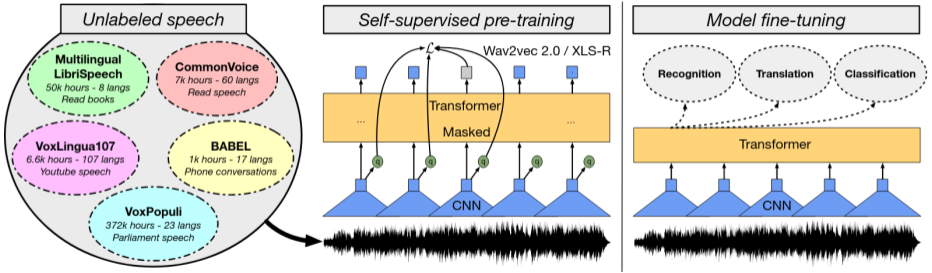
\includegraphics[width=10cm]{wav2vec2.png}
    \centering
    \label{fig:wav2vec2architecture}
    \caption{Illustration of the Wav2Vec2 framework adapted from \textcite{baevskiWav2vec20Framework2020a}}
\end{figure} 

\numberedparagraph{XLSR}
Using the above framework, \textcite{conneauUnsupervisedCrosslingualRepresentation2020} introduced the XLSR Wav2Vec2 model pretrained on multiple languages, with \textcite{babuXLSRSelfsupervisedCrosslingual2021} introducing several well known checkpoints of XLSR models pretrained on 53 languages at three different sizes of 300 million parameters, 1 billion parameters, and 2 billion parameters often short-handed as 300m, 1B, and 2B variants respectively. After pre-training on unlabeled data, it can be fine-tuned with \gls{ctc} loss \parencite{gravesConnectionistTemporalClassification} on a much smaller set of labeled data, achieving state-of-the-art results in scenarios where labeled data is scarce \textcite{baevskiWav2vec20Framework2020a}. These processes can be seen in Figure \ref{fig:wav2vec2architecture} adapted from \textcite{babuXLSRSelfsupervisedCrosslingual2021}.\todo{adapt diagram from wav2vec2 paper and explain the components properly.}


\chapter{Related Work}\label{ch:rw}
In the following section, we will dive into some existing strategies for overcoming data scarcity in \gls{md}. These approaches can be broadly split into two groups: attempts to eliminated dependency on the scarce \gls{l2} data entirely \parencite{korzekwaWeaklysupervisedWordlevelPronunciation2021}, or through generating the desired \gls{l2} data through various synthesis or augmenting techniques \todo{see l2gen for some of the papers supporting this split}. This delineation echoes the approaches to data scarcity for low-resource languages outlined in \ref{lr_scenarios}, and both avenues will be explored in the current work. We will start with an anchoring in recent applications of \gls{e2e} \gls{asr} in \gls{md} before exploring the specific ways the current work pursues overcoming data scarcity in relation to these two overarching strategies, specifically through: 
\begin{enumerate}
  \item \gls{asr} model ensembles,
  --and--
  \item \gls{tts}-generated data augmentation
\end{enumerate}
The former will serve as our exploration into knowledge transfer to circumvent the need for scarce \gls{l2} data, where the latter instead investigates the ability to overcome this scarcity directly through data synthesis.
\section{\gls{e2e} \gls{asr} for \gls{md}}
Following the general trend in \gls{asr} and \gls{ml} more broadly, 

\numberedparagraph{Touch on phoneme extraction task and detail fine-tuning procedure}
\textcite{agrawalLearningWhenTrust2023} smart weighter mechanism that selects model based on input audio

\numberedparagraph{MDD scoring}

% forest package for more painless trees
\begin{figure}[t]
\centering
\begin{adjustbox}{max width=\linewidth}
\begin{forest}
for tree={
  edge={-{Latex[length=1.6mm]}},
  l sep=5mm,        % level separation (vertical)
  s sep=2mm          % sibling separation (minimum horizontal)
}
[Transcribed Phonemes, internal
  [Correct Pronunciations, internal
    [True Acceptance, posleaf]
    [False Rejection, negleaf]
  ]
  [Mispronunciations, internal
    [False Acceptance, negleaf]
    [True Rejection, internal
      [Correct Diagnosis, posleaf]
      [Diagnosis Error,  negleaf]
    ]
  ]
]
\end{forest}
\end{adjustbox}
\label{fig:eval}
\caption{Evaluation hierarchy of phoneme level \gls{md}}
\end{figure}


\section{\gls{asr} Ensembling Strategies}

% https://developer.nvidia.com/blog/entropy-based-methods-for-word-level-asr-confidence-estimation/

\parencite[inter alia]{barteldsMakingMoreLittle2023,zhangL2GENNeuralPhoneme2022,kheirAutomaticPronunciationAssessment2023,thaiSyntheticDataAugmentation2019}
\numberedparagraph{how ensembling improves performance, different types}
As covered more extensively in the previous chapter, the state of modern \gls{ml} has seen a proliferation of models trained on massive amounts of data tuned to perform well on a variety of target tasks, but can still struggle to perform satisfactorally outside their domain of expertise. One long-standing general strategy for overcoming the limitations of any single classifier model in \gls{asr} as in \gls{ml} more generally is through \textit{ensembling}. In general terms, an ensemble refers to a set of classifiers whose outputs are combined in some way \parencite{dietterichEnsembleMethodsMachine2000}. Doing so effectively requires that these classifiers be similar in function but complementary in someway, being diverse enough to cover each other's weaknesses \parencite{hansenNeuralNetworkEnsembles1990}\todo{check source for their wording}. Originally, ensembles combined outputs of constituent models through Bayesian averaging, i.e. weighing the output of the model by the posterior probability of the output, giving each model what amounts to a weighted vote in the output \parencite{dietterichEnsembleMethodsMachine2000}. Despite this mathematically principled origin, it proved to be prohibitively time consuming to calculate for complex problems, and so alternatives were introduced which were more computationally tractable. A wide range of ensembling techniques have emerged over the years, including boosting, bagging, stacking, majority voting and confidence voting, all of which have proven robust methods of improving performance on a variety of tasks \parencite[see][inter alia]{maclinEmpiricalEvaluationBagging1997,dengScalableStackingLearning2012,fiscus1997post,gitmanConfidencebasedEnsemblesEndtoEnd2023}. For \gls{asr}, these approaches have yielded improvements over singular models with combinations of different model architectures \parencite{arunkumarInvestigationEnsembleFeatures2022,dengEnsembleDeepLearning2014}, and different training data such as for specific languages or dialects \parencite[inter alia]{agrawalLearningWhenTrust2023,gitmanConfidencebasedEnsemblesEndtoEnd2023}.

\numberedparagraph{existing work in the area, gaps}
An early example of an equal weight, majority voting-based system in \gls{asr} is \gls{rover} \parencite{fiscus1997post}, which aligns multiple systems with eachother to then vote on each aligned word slot, producing an aligned output string reached by model concensus. More dynamic approaches on the same theme have been explored as with \textcite{agrawalLearningWhenTrust2023}, whereby a weighting module is trained on transcriptions to select expert models so as to to minimize \gls{wer}, leading to an improvement over equal-weight voting. A number of confidence-based approaches have been taken towards language identification for both \gls{hmm} and more modern \gls{e2e} architectures \textcite{gitmanConfidencebasedEnsemblesEndtoEnd2023}, whereby only the outputs of the most confident model from the ensemble are used. One issue with deriving reliable confidence measures for modern \gls{e2e} \gls{dnn}-based models lies in their tendency toward overconfidence in ouptput predictions \parencite{weiMitigatingNeuralNetwork2022}, though some mitigation strategies have been introduced to derive more reliable confidence estimates from entropy calculations \parencite{laptevFastEntropyBasedMethods2023}. Ensembles have been utilized in a number of ways for phone-level \gls{md} as well. \textcite{ananthakrishnanUsingEnsembleClassifiers2011} investigated \gls{md} with a series of binary classifiers to detect mispronunciations typical of Swedish learners of varying \gls{l1} backgrounds, focusing on systematic phoneme confusion patterns over several utterances and exeplifying through two case studies how this approach could be used to motivate targeted interventions. \textcite{calikEnsemblebasedFrameworkMispronunciation2023a} also pursued \gls{md} for Arabic phonemes using a variety of model architectures and combination techniques i.e. bagging, boosting, stacking, and majority voting, finding majority voting the most performant.  

\numberedparagraph{Contribution of current work}
Although model ensembling has a long history in \gls{ml} and \gls{asr}, confidence-based ensembled have not to our knowledge been leveraged toward phone-level \gls{md}. Despite the relative scarcity of ensembling applications in \gls{md}, the limitations of data and model expertise motivating general ensemble applications clearly apply to \gls{l2}-speech-specific phone classifiers as well: monolingual data to train expert models for Irish and English is available in abundance, but phonetically labeled data for Irish \gls{l2} speakers with an English \gls{l1} is not so plentiful. Models tuned to output phones for English would not be expected to reliably transcribe Irish-specific phones, and models tuned to Irish would similarly underperform for English phones. But given the possibility of combining these expert systems in an ensemble, could each constituent expert model's phone coverage be leveraged to complement the other's towards identifying mispronunciations in Irish \gls{l2} speech? If combined as a confidence-based ensemble of monolingual expert systems, we might for example expect an English model to more confidently predict English-like phones in an attempted Irish utterance with heavy interference from the speaker's \gls{l1}, while a more native-like pronunciation for other segments without any \gls{l1} interference might be confidently transcribed by the Irish \gls{asr}. If we choose the most confidently predicted phone from each frame, we might be able to derive a combined string that more accurately reflects the segmental errors present in learner speech than is possible for each model on its own. 

\section{Data Generation with Synthetic Speech}
\todo{is augmenting my dataset with synthetic speech augmentation or data synthesis? both?}
On the other end of common solutions to \gls{l2} data scarcity, we encounter \textit{data augmentation} and \textit{data generation}. Data augmentation is frequently done through labeling of existing audio \parencite[see][inter alia]{xuIterativePseudoLabelingSpeech2020,yangImprovingMispronunciationDetection2022,barteldsMakingMoreLittle2023} or altering existing audio through targeted alternations to phonemes or other perturbations \parencite{kheirAutomaticPronunciationAssessment2023}.Automated labeling of unlabeled audio presents a promising avenue for low-resource languages, as it is easier to collect this kind of data than manually annotated data \parencite{barteldsMakingMoreLittle2023}, and for languages with at least some digital presence, there may be latent reservoirs of this kind of data available to propel such an approach. In \gls{asr} generally, \textcite{hayashiBackTranslationStyleDataAugmentation2018} pursued back-translation-like data augmentation was demonstrated to bolster performance, whereby a text-to-encoder translation model is trained to predict \gls{asr} hidden states, then using these to retrain the decoder without need for any speech paired to the augmenting text data. For \gls{mdd}, \textcite{yangImprovingMispronunciationDetection2022} illuminated the use of momentum pseudo-labeling via a teacher-student model ensemble using Wav2Vec2 as a promising way to leverage plentiful unlabeled \gls{l2} speech for improving \gls{mdd} performance.

In recent years, however, as end-to-end \gls{asr} models like Wav2Vec2 become increasingly capable, so to do their \gls{tts} counterparts, advancing to the point where the speech they produce is nearly indistinguishable from humans in naturalness. This development has led a number of researchers to pursue synthetic data generation via \gls{tts} as another way to fill the data gap for low-resource \gls{asr} \parencite[see][inter alia]{barteldsMakingMoreLittle2023,thaiSyntheticDataAugmentation2019,fazelSynthASRUnlockingSynthetic2021}. Use of \gls{tts} outputs to augment data has been demonstrated to provide improvements in \gls{wer} for \gls{asr} \parencite{barteldsMakingMoreLittle2023}, with the caveats that not all languages have readily available \gls{tts} systems. For \gls{mdd}, however, this inequality in \gls{tts} availability is less of an obstacle to providing useful data. The task of generating mispronunciation data has been framed in recent years by \textcite{korzekwaComputerassistedPronunciationTraining2022} and \textcite{zhangL2GENNeuralPhoneme2022} as \textit{phoneme paraphrasing}, as an analogue to the paraphrasing task in \gls{nlg}. The former approach by \textcite{korzekwaComputerassistedPronunciationTraining2022} proposes three avenues for synthesis---\gls{p2p}, \gls{tts}, and \gls{s2s}---all improving accuracy in detecting mispronunciation errors. The latter approach focuses on a \gls{p2p} pipeline, where canonical phone strings are translated to \gls{l2}-like variants using a \gls{s2s} \gls{mt} model, which is then diversified using their \gls{dpad} module to improve generalizability, and finally fed to a \gls{tts} system \gls{l1} to generate \gls{l2}-like mispronounced audio. Critically, a seed set for training the \gls{s2s} paraphraser was extracted from the expertly-annotated dataset used L2-arctic.

\textcite{punjabiLanguageModelBootstrapping2019} bootstrapping data with MT (important)
\textcite{xuIterativePseudoLabelingSpeech2020} multiple iteration of pseudo-labeling on unlabeled data to overcome data scarcity
\textcite{yangImprovingMispronunciationDetection2022} pseudo-labeling to overcome scarcity (self-superviced learning)

\textcite{khareLowResourceASR2021a} transliteration as a bridge between orthographies
\textcite{korzekwaComputerassistedPronunciationTraining2022} synthesis approaches to boosting asr
\textcite{barteldsMakingMoreLittle2023} TTS + ASR boosts ASR performance
\textcite{zhangL2GENNeuralPhoneme2022} phoneme paragraphing to generate mispronounced speech (important)
\numberedparagraph{experiment 2, gaps and contributions}
Similar to \textcite{zhangL2GENNeuralPhoneme2022} we see the potential for synthetic data as a possible answer to \gls{md} data scarcity through phone-to-phone translation to create controllable errors mirroring what one would expect from language learners with the same \gls{l1} the \gls{tts} is tailored to. Mapping phonetic transcriptions of canonical Ulster pronunciations to inputs acceptable to an English \gls{tts} gives highly English-sounding approximations of Irish speech with exactly the kinds of segmental errors one expects from English \gls{l1} learners of Irish\footnote{Another noteworthy property of the recordings is the English-like prosody and stress patterns, which could be pursued in an investigation into suprasegmental deviation from Ulster speech, but lies outside the scope of the current work.}. Instead of using a \gls{nn}-based architecture for our phone-to-phone paraphrasing, we use \gls{mfa} \gls{g2p} to hopefully improve performance with little data. Additionally, as we don't have an expertly annotated seed corpus to draw from with Irish as their work does by drawing the seed data from L2-arctic, we draw our seed data from Irish and English \gls{asr} outputs, an approach which we will elaborate on in the following chapter.\todo{revisit this sentence. I think the real change is more how we build our seed set}. L2-gen provides greater diversity through their DPAD augmentation system, but in the interest of time, we do not attempt here to introduce additional variance to the \gls{tts} voices, though we recognize this innovation as a critically important one for promoting more robust performance.

\chapter{Methods \& Materials}
In the following chapter, we will elaborate the core experiments explored for the current work: one which explores model ensembling as described above as a solution to \gls{md} in the face of data scarcity; the other, which explores data augmentation via bootstrapping \gls{tts} input with \gls{g2p} model to create the data required to train an \gls{asr} model directly for \gls{md}. We will begin with detailing the features in common between these experiments, and end with the evaluation details shared between experiments.\todo{maybe setup links to refer to research questions or sections}
\section{General Experiment Setup}
\todo{revisit connections to related work after that section is hammered out.}
At a high level, both of the \gls{md} pipelines explored follow the same general flow, starting with audio input of \gls{l2} speakers speaking Irish. The input waveform is then processed by one or several \gls{asr} models, configured to output strings of phonemes. These phoneme strings are then aligned to gold-standard transcriptions of the target string, allowing us to validate the performance of the \gls{asr} configuration through \gls{cer}. This string, together with derived posterior probabilities for frames corresponding to phonemes in the string, is used to compute \gls{gop} scores for the string's constituent phonemes, allowing us to gauge pronunciation quality.\todo{definitely don't feel like i understand }

\numberedparagraph{base model description}
The model chosen for all experiments was the 300 million parameter version of Wav2vec2 XLS-R \parencite{babuXLSRSelfsupervisedCrosslingual2021}. This choice of architecture was motivated by the desire to leverage the aforementioned pre-training/fine-tuning paradigm on a model shown by \textcite{babuXLSRSelfsupervisedCrosslingual2021} to improve on previous work most notably for low- and mid-resource languages. Selection of the 300 million parameter version of this architecture was primarily motivated by desire to rapidly train models and test ideas, aiming for proof-of-concept over beating the state-of-the-art. These models were fine-tuned on phonetically annotated datasets, allowing us to obtain phoneme-level transcriptions for comparison.

All models were implemented using the Hugging Face \textit{Transformers} library \parencite{wolfTransformersStateoftheArtNatural2020}. Training was managed with the Transformer \textit{Trainer} class, configured via \textit{TrainingArguments}. Training progress and metrics were logged to Weights \& Biases\todo{configure bibtex entry}. Our implementation of Wav2Vec2 for phoneme output followed the publicly available tutorial by Vitouphy on Kaggle \todo{how to cite this appropriately}. Models were instantiated with an attention dropout of 0.1, layer dropout of 0, feature projection dropout of 0, mask time probability of 0.75, mask time length of 10, mask feature probability of 0.25, and mask feature length of 64. \todo{create table with all this info}.

Training for all \gls{asr} models models used identical parameters, with batch size of four, learning rate 3e-5, 2000 warmup steps, and 16-bit precision training to reduce memory usage and speed up training. \gls{cer} was used in guiding early stopping, which had a patience of 6 epochs with a maximum of 30 epochs of training. \todo{create table with info. alternatively move this to the beginning to the other table if training is uniform (it should be)}

\section{Experiment 1: Monolingual Model Ensembling} \label{ex:1}
\numberedparagraph{outline first experiment with model ensemble.}
Our first experiment starts with the ensembling intuition described above\todo{maybe reference ensembling section} using two\todo{three if using russian?} expert systems: one Irish and one English. In contrast to previous works like \textcite{dengEnsembleDeepLearning2014}\todo{what was i saying here?}. To yield posterior probability-like values from these model outputs, logit outputs of each model are normalized across the output vector for each frame. These normalized frame vectors are then compared to eachother with a heuristic selection mechanism: for every frame in the output vector, this block compares each component model output for that frame, and simply selects the model output with highest confidence. The combined output is then decoded, yielding a combined output string of phonemes with corresponding confidence values to be used at evaluation.

\textcite{guoCalibrationModernNeural2017} predicting probability estimates. how well calibrated are our models?
\textcite{niehuesModelingConfidenceSequencetoSequence2019} similarity between training and test conditions for confidence (maybe more suitable as an extension)
\textcite{papadopoulosConfidenceEstimationMethods2001} maximum likelihood, approximate bayesian, bootstrapping. (confidence estimation assessed by mean and st dev etc.)
\textcite{weiMitigatingNeuralNetwork2022} mitigating overconfidence with logit normalization during training. some background on softmax confidence scores

\subsection{Data}
\numberedparagraph{briefly summarize data sources}
To train our monolingual systems, we procured two monolingual corpora of read speech audio with phonetic transcriptions. Our English model was trained on the TIMIT corpus \textcite{garofoloDARPATIMITAcousticphonetic1993} with the Irish model trained on audio data from the online Irish Dictionary and Language Library\footnote{\url{https://www.teanglann.ie/en/}}. 
\textcite{krishenbaumRepresentingIPAPhonetics} use if ascii is used (it's not)
\textcite{mechuraIntroductionGramadanIrish} introduction to grammar part of teanglann (not relevant? what did i want this for again?)

\subsubsection{timit}
The TIMIT corpus is a read speech corpus of American English speakers who spent their childhoods in one of eight major dialect areas of the United States. These areas are widely recognized with the exception of the Western dialect region, where boundaries are not confidently delineated, and the "army brat" group, consisting of speakers which frequently moved during their childhood due to the demands of highly mobile military service member parents, resulting in exposure to a variety of dialects\parencite{garofoloDARPATIMITAcousticphonetic1993}. The full dataset consists of 6300 sentences from 630 speakers, so ten sentences per speaker. The duration of the data loaded from the Kaggle dataset linked to the TIMIT github dataset\footnote{https://github.com/philipperemy/timit} lies at two hours and forty minutes. The TIMIT phonetic transcriptions were given in a revised version of ARPABET, a set of transcription codes developed by Advanced Research Projects Agency (ARPA)\todo{dig up reference for this}. 

\subsubsection{teanglann}
The Dictionary and Language Library is an online resource developed by Foras na Gaeilge\footnote{Foras na Gaeilge is a group which promotes the Irish language, supports Irish-medium education, and advises public and private sector organizations, among its other functions. \url{https://www.forasnagaeilge.ie/}} in conjunction with the New English-Irish Dictionary. Among the resources available are The Pronunciation Database, which contains recordings of individual words spoken by native speakers from three major dialects: Connacht, Ulster, and Munster. The Ulster recordings used for our monolingual Irish model were scraped by myself, adhering to the site's robots.txt file limit of one request per two seconds. The words scraped were drawn from an available \gls{g2p} dictionary\todo{maybe elaborate more where this comes from} to ensure scraped audio had a corresponding canonical \gls{ipa} transcriptions\footnote{The dictionary of words to scrape was derived from an Ulster Irish \gls{g2p} file generously provided by Jim O' Regan}. The resultant combined dataset had an audio duration of roughly five hours of audio.
\todo{talk to jim about where he got the g2p dict I use for pronunciation information and as a scraping dict}

\subsubsection{Preprocessing}
The audio from both Teanglann and TIMIT was loaded and resampled to 16kHz for compatability with Wav2vec2. For the phonetic trancriptions, TIMITs phonetic representations were translated to IPA using the phonecodes library, and maintaining one space between each phoneme or dipthongs\footnote{dipthongs were kept together as a single single unit to keep with standard practice}. The Irish data was transcribed through a lookup in the aforementioned \gls{g2p} dictionary, which adhered to the same spacing rules as for TIMIT.

\subsection{Experimental Setup}
We split the datasets into train/dev/test splits with .8/.1/.1 ratios respectively, and then trained according to the above common . One critical limitation with the Irish data was that due to the acquisition method, we were left with no way verifiable way to identify speakers, so the different splits likely contains speaker overlap. We sought to mirror this limitation with the English data so as to not bias any particular language when ensembling them, and so the monolingual evaluation metrics are also likely overly optimistic. 

\section{Experiment 2: Synthetic Mispronunciation Data}
\todo{rework section to reflect change in approach from iterative bootstrapping to asr confusion mapping.}
The second experiment set out to capture mispronunciation by training a single \gls{asr} model whose base training data of more readily available, correctly pronounced native-speaker data was augmented with learner-like \gls{tts}-generated mispronounced versions of this base dataset. The input for generating this learner-like synthetic data is obtained through an iterative manual bootstrapping method whereby initial phonetic transcriptions of a set of words are adjusted to produce reasonable learner-like attempts to pronounce the canonical versions of each utterance via \gls{ssml} input to the \gls{tts} system. These manually adjusted transcriptions are then used to train a \gls{g2p} model, from which we obtain a new round of phonetic transcriptions for the next set of words. The adjust-train-generate process is repeated until automatically generated transcriptions need only minimal if any adjustments.

\subsection{Data} 
Canonical pronunciations were obtained from the Teanglann pronunciation dictionary, with corresponding canonical \gls{ipa} transcriptions from the aforementioned Ulster Irish \gls{g2p} dictionary: the same dataset as that used for training the Irish model in Experiment \ref{ex:1}. The augmenting learner-like recordings were obtained from Google Cloud \acrlong{tts}\todo{what to reference for this service?} using the \todo{mention voice(s) used here} voice(s) at a recording frequency of 16kHz\todo{double check the frequency}. The input was given in \gls{ssml} to enable direct use of \gls{ipa} transcriptions to guide pronunciation. These correctly pronounced and corresponding mispronounced synthetic samples of each word composed the \textit{positive} and \textit{negative} utterance pairs of the training data. \todo{I will likely circle back to this distinction in the discussion section when suggesting an extension for contrastive training}

\subsection{Experimental Setup}
Input was given as \gls{ipa} strings in \gls{ssml} format, 
The iterative improvement of \gls{tts} inputs was carried out by manual improvements of \gls{mfa} \gls{g2p} \parencite{mcauliffeMontrealForcedAligner2017} in batches of 50 utterances at a time between retraining using default parameters\todo{is there anything interesting I can say about these models?}. This process was repeated x times \todo{remember to complete this with the actual number of iterations}, at which point the \gls{g2p}-generated transcriptions ceased to improve meaningfully and required no changes to yield plausible learner speech.
After training the above \gls{g2p} model, recordings were produced from the \gls{tts} service for the remaining instances not used in \gls{g2p} training. These recordings along with the \gls{ipa} strings used to produce them were combined with aforementioned Teanglann recordings and their canonical transcriptions.

\section{Evaluation}
We evaluate phone-level discrimination of the \gls{asr} by first aligning model output strings to the \textit{gold standard} annotated sequence with the Needleman-Wunsch algorithm \parencite{needlemanGeneralMethodApplicable1970} using the \gls{nltk} library \todo{complete with whatever library I use for this.}. From this alignment we can then compute \gls{per} F1, Recall, \todo{all the other crap} 
model off \parencite{leungCNNRNNCTCBasedEndtoend2019}


\subsection{Metrics}
For assessing the match of \todo{what am I using in my comparisons?}
\todo{statistcal testing?}

\subsection{Data}
\numberedparagraph{Common voice}
For evaluating the quality of our \gls{md} systems' sensitivity to plausible Irish \gls{l2} errors, we first needed Irish \gls{l2} speech. We begin with the Irish portion of the Common Voice dataset\textcite{ardilaCommonVoiceMassivelyMultilingual2020}, noted by \textcite{lonerganAutomaticSpeechRecognition} as consisting nearly entirely of \gls{l2} speakers\footnote{given its nature as a crowd-sourced dataset, some data has been added since that date, but its character as a largely if not entirely \gls{l2} speaker-dominated set of Irish speech should remain the case}. As in their work, this dataset will be used as the basis for testing the current experiment, as it fits the purpose of evaluating our system's effectiveness on \gls{l2} speech. The Common Voice corpus is a massive multilingual collection of transcribed speech designed for \gls{asr} which leverages crowd sourcing for data collection and validation to help alleviate the dirth of training data faced by most languages. \todo{why do I have three of the same paragraph} \todo{common voice used in wav2vec2 xls-r pretraining. they use the december 2020 checkpoint. use data after this for eval.}

\numberedparagraph{annotation details} 
To prepare the Common Voice dataset for use in phoneme-level \gls{md}, a small subset of the data was manually transcribed in \gls{ipa} to capture pronunciation deviations from standard Ulster pronunciation. The process of capturing these deviations consisted of the following steps: first, an \gls{ipa} representation of the transcription was generated from a lookup in the Ulster \gls{g2p} dictionary to map the orthographic transcriptions to their canonical \gls{ipa} representations; recordings were then manually assessed, comparing these generated \gls{ipa} representations to the audio and noting where the phonemes deviated from the canonical pronunciations and what their realization was assessed to be. This process was carried out by myself only, a notable limitation we will return to later. The annotations were carried out in Label Studio using some preliminary annotations generated by a lookup in the aforementioned Ulster \gls{g2p} dictionary with a \gls{mfa} \gls{g2p} model trained on this dictionary to serve as a fallback when the lookup returned no match.\todo{ask about where the g2p dict came from, what to reference}

\textcite{conneauFLEURSFewshotLearning2022} Parallel ASR dataset. move to discussion.
\textcite{deichlerMMConvMultimodalConversational2024} multimodal conversational dataset with cospeech gestures. move to discussion
\textcite{qianAutomaticSpeechRecognition2022} ASR for irish: uses Mozilla common voice
\textcite{zhangSpeechocean762OpenSourceNonnative2021} open source speech corpus speech ocean for pronunciation assessment
\textcite{zhaoL2ARCTICNonnativeEnglish2018} L2 arctic dataset
\textcite{leeMassivelyMultilingualPronunciation} wikipron (not used but illustrative as a reference)
\numberedparagraph{metrics CER, F1, etc. Detail CTC loss used in training}
CTC loss \textcite{gravesConnectionistTemporalClassification} also details some peakiness
\textcite{kurzingerCTCSegmentationLargeCorpora2020} ctc and dataset bootstrapping (maybe not relevant with shift from bootstrapping to 1-shot paraphrasing)

\subsection{Skyline Comparison}
To see how our approaches compare to more idealize skyline conditions we compare performance of the above experiments to the average performance of four models trained on English \gls{l2} speakers with a commonly used dataset for \gls{md} research: L2ARCTIC \parencite{zhaoL2ARCTICNonnativeEnglish2018}. L2-ARCTIC is a read-speech corpus of non-native English, originally released with speakers of five different \glspl{l1}: Hindi, Korean, Mandarin, Spanish, and Arabic, though Vietnamese has since been added. At present, each language has four speakers: two male and two female, from whom over an hour of speech recordings were taken along with word- and phoneme-level transcription, and selected manual annotations for each recording. 
To train our skyline models, we confined ourself to one speaker \gls{l1} group, Spanish. This was to allow our models to learn a single \gls{l1} interference profile relatively close to English while minimizing heterogeneity in \gls{l1} interference \todo{Still not sure what I think about this sentence}. The phoneme-level annotations were presented in ARPABET, from which we could obtain \gls{ipa} phonetic transcriptions to train models using the same training strategy outlined above. Due to the limited speaker pool of four for each language, and within that, two for each gender, any one model trained with a held out speaker for evaluation ran the risk of overfitting to a specific gender profile. To combat this, we ran 4-fold \gls{loso} \gls{cv}, using the average performance to represent our skyline performance ceiling.

\chapter{Results}
\numberedparagraph{detail the results as it pertains to the evaluation framework: CER, MDD metrics, etc}


\chapter{Discussion}
\numberedparagraph{Summarize the main findings from results and how it relates to the research questions}
\parencite{conneauUnsupervisedCrosslingualRepresentation2020} low-resource languages benefit more from similar higher-resource languages.

\numberedparagraph{why confidence might need adjusting?} \parencite{laptevFastEntropyBasedMethods2023}

\numberedparagraph{Detail possible applications to Language learning, the role of results in augmenting self-directed language learning}
\textcite{hardisonSecondlanguageSpokenWord2005} effect of multimodal input on speech identification

\numberedparagraph{Detail possible (or actual if time allows) Furhat application} 
\textcite{deichlerMMConvMultimodalConversational2024} multimedia data

\numberedparagraph{continue furhat explanation}

\numberedparagraph{Argue for accurate articulator representation in digital agents as supportive pillar in pronunciation feedback.}
%\textcite{Li2011ThePA} Animated articulators
\textcite{rosenblumSpeechPerceptionMultimodal2008} speech perception as multimodal phenomenom

\chapter{Conclusions}
\numberedparagraph{reiterate how results connect with research questions, set main conclusions in context of impact to research and society}
\textcite{zeyerWhyDoesCTC2021} peaky ctc, ambiguous phone boundaries

\numberedparagraph{Extensions from previous research (yang2022)}
\textcite{liuEndtoEndUnsupervisedSpeech2023} wav2vec which does adversarial training to improve discrimination.
\textcite{pengEndtoEndMispronunciationDetection2023} contrastive loss optimization
\textcite{lonerganLowresourceSpeechRecognition2024} alternative architectures for low resource asr
\textcite{neriEffectivenessComputerAssisted2008} pronunciation training for children, lead to improvements comparable to traditional training
\textcite{prabhavalkarMinimumWordError2017} alternatives to ctc

\numberedparagraph{Possibilities for future work}
\textcite{gongTransformerBasedMultiAspectMultiGranularity2022} assessment targeting more than one aspect of speech (prosody, word-level stress)
\textcite{mortensenPanPhonResourceMapping} PanPhon mapping from ipa to articulatory features
\textcite{rouditchenkoComparisonMultilingualSelfSupervised2023} language family in pretraining predictive of how models compare. need for resources for smaller families
\textcite{sjons2022articulation} focus on child directed speech, since it is well-suited for word segmentation?

\chapter{Ethical Considerations}
\numberedparagraph{General Ethical considerations for current work and possible extensions}

\numberedparagraph{Ethical considerations for Minority languages}

\chapter{AI Tools}
\numberedparagraph{Describe use of AI tools and how its use benefited me.}

\appendix
\printbibliography
% at start yields errors because there are no citations and the bibliography file is empty
\end{document}
